\chapter{Conclusion}
brief of conclusion

\section{Conclusion of Problems}
Tell about solving the problem

\section{Conclusion of Method}
Tell about solving using method

\section{Conclusion of Experiment}
Tell about solving in the experiment

\section{Conclusion of Result}
tell about result for purpose of this research.

\section{Yusniar Nur Syarif Sidiq/1164089}
\subsection{Pemahaman Teori / Yusniar Nur Syarif Sidiq / 1164089}

\begin{enumerate}

\item Jelaskan kenapa kata-kata harus dilakukan vektorisasi. Dilengkapi dengan ilustrasi atau gambar.
	\subitem Dikarenakan mesin hanya mampu membaca data dengan bentuk angka maka dari itu diperlukan vektorisasi kata atau bisa disebut dengan mengubah kata menjadi bentuk vektor agar mesin seolah-olah paham apa yang kita maksudkan. Kal inii saya memberikan ilustrasi sederhana, dimana ada sebuah data mengenai kucing, tikus, dan pulpen. Bagaimana cara mesin untuk membaca data tersebut ?, yaitu dengan cara dilakukannya vektorisasi kata. Fungsi dari vektorisasi itu sendiri ialah sebagai indentitas, misalnya di dalam dokumen kucing terdapat kata-kata yang sudah di vektorisasi dan hasilnya adalah 0.012,0.024,.....,0.300, pada dokumen tikus menghasilkan 0.015,0.026,....,0.0276, dan pada pulpen menghasilkan -0.191,...,-0.045. Data vektor tersebut merupakan identitas dari data kucing, tikus dan pulpen.Apabila nilai vektor cenderung sama, maka data tersebut memiliki similarity atau data yang memiliki konten kata yang sama akan tetapi berbeda dengan pulpen yang memiliki data vektorisasi minus, sehingga dapat disimpulkan pulpen memiliki konten kata yang berbeda. Dengan adanya vektorisasi tersebut maka mesin seolah-olah mengerti bahwa kucing dan tikus memiliki konten yang sama yaitu merupakan objek dari binatang sedangkan pulpen merupakan objek benda mati. Mengenai contoh gambarnya dapat dilihat pada figure \ref{YNC5-1}

	\begin{figure}[ht]
		\centering{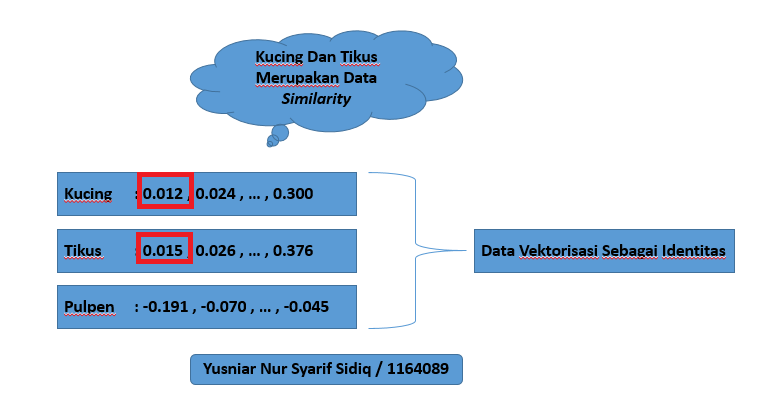
\includegraphics[scale=0.5]{figures/YN/Chapter5/Teori/YNC5-1.png}}
		\caption{Kata-Kata Hasil Vektorisasi}
		\label{YNC5-1}
	\end{figure}

\item Jelaskan mengapa dimensi dari vektor dataset google bisa sampe 300. Dilengkapi dengan ilustrasi atau gambar.

\item Jelaskan konsep vektorisasi untuk kata. Dilengkapi dengan ilustrasi atau gambar.

\item Jelaskan konsep vektorisasi untuk dokumen. Dilengkapi dengan ilustrasi atau gambar.

\item Jelaskan apa mean dan standar deviasi. Dilengkapi dengan ilustrasi atau gambar.
	\subitem Mean merupakan nilai rata-rata dari suatu data. Mean dapat dicari dengan cara membagi jumlah data dengan banyak data sehingga diperoleh lah nilai rata-rata dari suatu data. Sedangkan standar deviasi merupakan sebuah teknik statistik yang digunakan dalam menjelaskan homogenitas kelompok.

\item Jelaskan apa itu skip-gram. Dilengkapi dengan ilustrasi atau gambar.
	\subitem Skip-gram merupakan sebuah teknik yang digunakan pada area speech processing yang dimana n-gram dibentuk lalu ditambah dengan tindakan skip.

\end{enumerate}